\documentclass[tikz]{standalone}

\usepackage{amsmath}
\usepackage{lmodern}
\usepackage{pgfplots}
\usepackage{physics}

\usetikzlibrary{arrows.meta}

\pgfplotsset{compat=1.17}

\definecolor{exotic orange}{RGB}{255,128,0}
\definecolor{exotic green}{RGB}{0,102,102}
\definecolor{exotic blue}{RGB}{0,202,161}
\definecolor{exotic red}{RGB}{250,86,86}

\begin{document}
	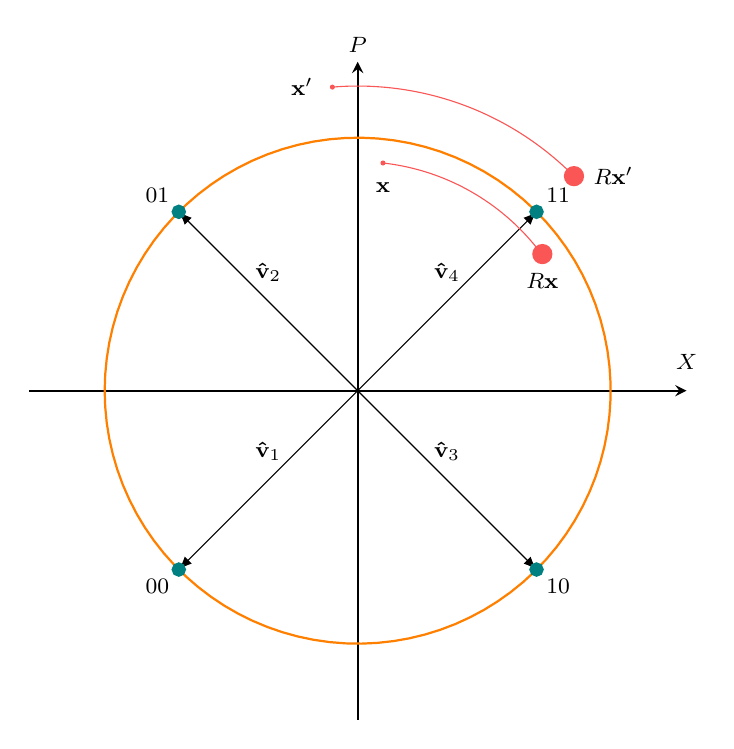
\begin{tikzpicture}[
		font=\fontsize{8}{9}\selectfont,
	]
		\begin{axis}[
			width=0.95\linewidth,
			axis lines=center,
			axis equal image,
			xlabel={$X$},
			ylabel={$P$},
			ticks=none,
			xmin=-1.3,
			xmax=+1.3,
			ymin=-1.3,
			ymax=+1.3,
			domain=-180:180,
			samples=100,
			axis line style={thick},
			x label style={
				at={(axis description cs:1,0.57)},
				anchor=north,
			},
			y label style={
				at={(axis description cs:0.5,1)},
				anchor=south,
			},
			cycle list name=exotic,
			every mark/.append style={solid},
		]
			\addplot+[very thick, only marks] coordinates {(0.707,0.707) (0.707,-0.707) (-0.707,0.707)(-0.707,-0.707)};
			\addplot+[thick, no markers] ({cos(x)},{sin(x)});
			\draw[-Latex] (axis cs:0,0) -- (axis cs:0.707,0.707) node[midway, label={$\vu{v}_4$}]{} node[above right]{$11$};
			\draw[-Latex] (axis cs:0,0) -- (axis cs:0.707,-0.707) node[midway, label={$\vu{v}_3$}]{} node[below right]{$10$};
			\draw[-Latex] (axis cs:0,0) -- (axis cs:-0.707,0.707) node[midway, label={$\vu{v}_2$}]{} node[above left]{$01$};
			\draw[-Latex] (axis cs:0,0) -- (axis cs:-0.707,-0.707) node[midway, label={$\vu{v}_1$}]{} node[below left]{$00$};
			
			\draw[draw=none, fill=exotic red] (axis cs:0.1,0.9) circle (0.01) node[label={below:$\vb{x}$}]{};
			\draw[draw=none, fill=exotic red] (axis cs:0.73,0.54) circle (0.04) node[label={below:$R\vb{x}$}]{};
			\addplot+[exotic red, domain=0:-45, no markers] ({0.1*cos(x)-0.9*sin(x)},{0.1*sin(x)+0.9*cos(x)});
			
			\addplot+[exotic red, domain=0:-50, no markers] ({-0.1*cos(x)-1.2*sin(x)},{-0.1*sin(x)+1.2*cos(x)});
			\draw[draw=none, fill=exotic red] (axis cs:-0.1,1.2) circle (0.01) node[label={left:$\vb{x}^\prime$}]{};
			\draw[draw=none, fill=exotic red] (axis cs:0.855,0.848) circle (0.04) node[label={right:$R\vb{x}^\prime$}]{};
		\end{axis}
	\end{tikzpicture}
\end{document}